\documentclass[11pt]{article}
\usepackage{fontspec}
\setmainfont{DejaVu Serif}
\setsansfont{DejaVu Sans}
\usepackage{polyglossia}\setmainlanguage{greek}\setotherlanguage{english}
\tolerance=2500\emergencystretch=3em
\usepackage{amsmath,amssymb}
\usepackage{geometry}\geometry{margin=2.4cm}
\usepackage{xcolor}\usepackage{graphicx}\usepackage{enumitem}\usepackage{booktabs}
\usepackage{caption}\captionsetup{font=small,labelfont=bf}
\usepackage[hidelinks]{hyperref}
\graphicspath{{figures/}}

\definecolor{ink}{HTML}{16212e}\definecolor{accent}{HTML}{1f5fa8}\definecolor{soft}{HTML}{eef3fb}
\definecolor{warn}{HTML}{a8341f}\definecolor{good}{HTML}{1f7a44}\color{ink}
\newcommand{\key}[1]{\par\medskip\noindent\colorbox{soft}{\parbox{\dimexpr\linewidth-2\fboxsep}{\textcolor{accent}{\textbf{Κλειδί:}}\ #1}}\par\medskip}
\newcommand{\ex}[1]{\par\smallskip\noindent\textbf{\textcolor{accent}{Παράδειγμα.}}\ #1\par\smallskip}
\newcommand{\warnb}[1]{\par\medskip\noindent\colorbox{soft}{\parbox{\dimexpr\linewidth-2\fboxsep}{\textcolor{warn}{\textbf{Προσοχή:}}\ #1}}\par\medskip}
\setlength{\parskip}{0.5em}\setlength{\parindent}{0pt}
\usepackage{titlesec}
\titleformat{\section}{\large\bfseries\color{accent}}{\thesection.}{0.5em}{}
\titleformat{\subsection}{\normalsize\bfseries}{}{0em}{}

\title{\textbf{\sffamily Σεμινάριο: Καταστάσεις πεποίθησης --- Kalman και BOCPD}\\[3pt]
\large Πώς το μοντέλο «καταλαβαίνει» τάση και αλλαγή καθεστώτος --- για αρχάριους}
\author{Dr.\ Stefanos Drakos \,\textemdash\, QUANTIQ / AGEL AI}
\date{Ιούνιος 2026}

\begin{document}
\maketitle\thispagestyle{empty}

\noindent
Στο προηγούμενο φυλλάδιο είδαμε το νευρωνικό δίκτυο LSTM. Εκεί αναφέραμε ότι δεν του δίνουμε ωμές
τιμές, αλλά \textbf{δέκα προεπεξεργασμένες πληροφορίες}. Τέσσερις από αυτές προέρχονται από δύο κομψά
εργαλεία: το \textbf{φίλτρο Kalman}, που εκτιμά την τάση και πόσο σίγουρη είναι, και το \textbf{BOCPD},
που εντοπίζει πότε αλλάζει το «καθεστώς» της αγοράς. Αυτές λέγονται \textbf{καταστάσεις πεποίθησης}
(belief states): δεν είναι η τιμή, είναι η \emph{εκτίμησή} μας για το τι συμβαίνει πίσω από την τιμή.
Αυτό το φυλλάδιο τα εξηγεί από το μηδέν, με αριθμητικά παραδείγματα.

\section{Το πρόβλημα: από τη θορυβώδη τιμή στην πεποίθηση}

Η ημερήσια τιμή είναι γεμάτη θόρυβο. Μια ανοδική μετοχή μπορεί κάλλιστα να κλείσει αρνητικά μια τυχαία
μέρα. Αν ταΐσουμε το μοντέλο με τη γυμνή τιμή, το αναγκάζουμε να ξεχωρίσει μόνο του το σήμα από τον
θόρυβο --- δύσκολο και ασταθές. Προτιμούμε να του δώσουμε απαντήσεις σε δύο συγκεκριμένες ερωτήσεις:
\begin{itemize}[nosep,leftmargin=1.4em]
\item \textbf{Προς τα πού πάει η αγορά, και πόσο σίγουρα;} --- το αναλαμβάνει το φίλτρο Kalman.
\item \textbf{Μήπως μόλις άλλαξε το παιχνίδι;} --- το αναλαμβάνει το BOCPD.
\end{itemize}

% ===================== KALMAN =====================
\section{Το φίλτρο Kalman: τάση με αυτοπεποίθηση}

Το φίλτρο Kalman είναι ένας «έξυπνος εκτιμητής» που, σε κάθε βήμα, συνδυάζει \textbf{τι περίμενε} με
\textbf{τι είδε} και βγάζει την καλύτερη δυνατή εκτίμηση. Το ίδιο μαθηματικό εργαλείο καθοδηγεί
διαστημόπλοια και GPS· εμείς το στρέφουμε στην τιμή.

\subsection{Η κατάσταση: επίπεδο και ταχύτητα}
Υποθέτουμε ότι πίσω από τη θορυβώδη τιμή κρύβονται δύο μεγέθη που δεν βλέπουμε άμεσα: το πραγματικό
\textbf{επίπεδο} (πού βρίσκεται η τιμή «καθαρισμένη» από θόρυβο) και η \textbf{ταχύτητα} (πόσο γρήγορα
ανεβαίνει ή κατεβαίνει). Τα μαζεύουμε σε ένα διάνυσμα κατάστασης $x=[\,\text{επίπεδο},\ \text{ταχύτητα}\,]$.
Το μοντέλο «τοπικά γραμμικής τάσης» λέει απλώς ότι το αυριανό επίπεδο ισούται με το σημερινό συν την
ταχύτητα, και η ταχύτητα αλλάζει αργά:
\[
\text{επίπεδο}_{t} = \text{επίπεδο}_{t-1} + \text{ταχύτητα}_{t-1}, \qquad
F=\begin{bmatrix}1&1\\[1pt]0&1\end{bmatrix},\quad H=\begin{bmatrix}1&0\end{bmatrix}.
\]
Ο πίνακας $H$ λέει ότι παρατηρούμε μόνο το επίπεδο (την τιμή), όχι την ταχύτητα --- αυτή πρέπει να την
\emph{συμπεράνουμε}.

\subsection{Ο κύκλος: πρόβλεψη και διόρθωση}
Σε κάθε μέρα το φίλτρο κάνει δύο κινήσεις. Πρώτα \textbf{προβλέπει} πού θα έπρεπε να είναι η τιμή με βάση
τη χθεσινή ταχύτητα. Μετά βλέπει την \textbf{πραγματική} τιμή και υπολογίζει τη διαφορά, που τη λέμε
\textbf{καινοτομία} (innovation) $\nu = \text{παρατήρηση} - \text{πρόβλεψη}$. Τέλος \textbf{διορθώνει}
την εκτίμησή του κατά ένα ποσοστό αυτής της διαφοράς· το ποσοστό λέγεται \textbf{κέρδος Kalman} $K$:
\[
x \leftarrow x + K\,\nu.
\]
Αν το φίλτρο είναι σίγουρο, το $K$ είναι μικρό (αγνοεί τον θόρυβο)· αν είναι αβέβαιο, το $K$ είναι
μεγάλο (μαθαίνει γρήγορα από τη νέα τιμή). Αυτή η ισορροπία προκύπτει \emph{αυτόματα} από την
αβεβαιότητα που το φίλτρο παρακολουθεί.

\subsection{Τι δίνουμε στο μοντέλο: τρεις αναγνώσεις}
Από αυτόν τον μηχανισμό βγάζουμε τρία καθαρά χαρακτηριστικά:
\begin{itemize}[nosep,leftmargin=1.4em]
\item \textbf{ταχύτητα} --- πόσο γρήγορη είναι η τάση.
\item \textbf{σημαντικότητα τάσης} $=\dfrac{\text{ταχύτητα}}{\sqrt{\text{αβεβαιότητα ταχύτητας}}}$ --- ένα
«t-στατιστικό»: μεγάλη ταχύτητα με μικρή αβεβαιότητα σημαίνει \emph{αξιόπιστη} τάση, όχι τύχη.
\item \textbf{τυποποιημένη έκπληξη} $=\dfrac{\nu}{\sqrt{\text{αβεβαιότητα παρατήρησης}}}$ --- πόσο
απρόσμενη ήταν η σημερινή κίνηση σε σχέση με ό,τι περίμενε το φίλτρο.
\end{itemize}

\ex{Έστω ότι το φίλτρο εκτιμά ταχύτητα $0{,}002$ ανά ημέρα με τυπική απόκλιση $0{,}0008$. Η
σημαντικότητα τάσης είναι $0{,}002/0{,}0008 = 2{,}5$ --- όπως ένα t-στατιστικό πάνω από $2$, δηλαδή μια
τάση που μάλλον είναι αληθινή και όχι θόρυβος. Αν αύριο η τιμή κάνει ένα απότομο άλμα, η «έκπληξη» θα
εκτιναχθεί, σινιάλο ότι κάτι ασυνήθιστο συμβαίνει.}

\key{Το Kalman δεν προβλέπει το μέλλον. Καθαρίζει το \emph{παρόν}: μετατρέπει μια θορυβώδη τιμή σε
«τάση συν βαθμός εμπιστοσύνης», που είναι πολύ πιο χρήσιμα για μια απόφαση.}

% ===================== BOCPD =====================
\section{BOCPD: πότε αλλάζει το καθεστώς}

Το Kalman είναι εξαιρετικό όσο η αγορά συμπεριφέρεται «κανονικά». Όμως κάθε τόσο το παιχνίδι
\textbf{αλλάζει} ριζικά --- ένα κραχ, μια αλλαγή πολιτικής, μια νέα φάση. Θέλουμε έναν ανιχνευτή που να
το πιάνει γρήγορα. Αυτό κάνει το \textbf{BOCPD} (Bayesian Online Changepoint Detection).

\subsection{Η ιδέα του «μήκους διαδρομής»}
Το BOCPD παρακολουθεί μια κρυφή ποσότητα: το \textbf{μήκος διαδρομής} $r_t$, δηλαδή \emph{πόσες μέρες
πέρασαν από την τελευταία αλλαγή καθεστώτος}. Επειδή δεν το ξέρουμε με βεβαιότητα, κρατάμε μια ολόκληρη
\textbf{κατανομή πιθανότητας} πάνω στο $r_t$: «πιθανότητα 70\% ότι είμαστε 40 μέρες στο ίδιο καθεστώς,
5\% ότι μόλις ξεκινήσαμε...».

Σε κάθε μέρα συμβαίνει ένα από δύο: είτε η τρέχουσα διαδρομή \textbf{συνεχίζεται} (το $r$ αυξάνεται κατά
ένα), με πιθανότητα $1-h$, είτε υπάρχει \textbf{σπάσιμο} και το $r$ μηδενίζεται, με πιθανότητα $h$ (το
$h$ λέγεται \emph{hazard}, π.χ.\ $1/250$ για ένα αναμενόμενο σπάσιμο ανά έτος). Το BOCPD ενημερώνει την
κατανομή ζυγίζοντας πόσο καλά η σημερινή τιμή ταιριάζει με κάθε σενάριο.

\subsection{Το σήμα: η μάζα πέφτει στα μικρά μήκη}
Όσο η αγορά είναι σταθερή, η πιθανότητα μαζεύεται σε \emph{μεγάλα} $r$ (είμαστε καιρό στο ίδιο
καθεστώς). Όταν συμβεί πραγματικό σπάσιμο, η σημερινή τιμή δεν ταιριάζει πια με τη μακρά διαδρομή, και
η πιθανότητα \textbf{καταρρέει απότομα στα μικρά $r$}. Αυτή ακριβώς η κατάρρευση είναι το σήμα μας. Το
ποσοτικοποιούμε ως \textbf{σοβαρότητα} (severity): τη συνολική πιθανότητα το μήκος διαδρομής να είναι
μικρό,
\[
\text{σοβαρότητα}_t \;=\; \Pr(r_t < k) \;=\; \sum_{r=0}^{k-1}\Pr(r_t=r), \qquad k=5.
\]
Κοντά στο $0$ σημαίνει «ήρεμα, καμία αλλαγή»· κοντά στο $1$ σημαίνει «μόλις άλλαξε το καθεστώς».

\ex{Σε μια ήρεμη ανοδική περίοδο η σοβαρότητα μένει χαμηλή (π.χ.\ $0{,}02$): όλη η πιθανότητα είναι σε
μεγάλα μήκη διαδρομής. Μόλις ξεσπάσει ένα κραχ, μέσα σε λίγες μέρες η σοβαρότητα εκτινάσσεται προς το
$0{,}8$+ --- το μοντέλο «καταλαβαίνει» ότι το προηγούμενο καθεστώς τελείωσε και γίνεται αμυντικό.}

\key{Γι' αυτό λέμε το BOCPD «έξυπνο φρένο»: δεν αντιδρά σε μία απλή πτώση τιμής, αλλά σε μια
\emph{αλλαγή της ίδιας της συμπεριφοράς} της αγοράς. Πατάει φρένο στις πραγματικές αλλαγές, όχι στον
καθημερινό τρόμο.}

\subsection{Μια τίμια λεπτομέρεια (που μας κόστισε ένα bug)}
Θα ήταν φυσικό να χρησιμοποιήσει κανείς ως ανιχνευτή την πιθανότητα $\Pr(r_t=0)$ --- «μόλις
μηδενίστηκε». Όμως, μετά την κανονικοποίηση, αυτή η ποσότητα ισούται \emph{πάντα} με το hazard $h$, εξ
ορισμού· δεν μεταφέρει καμία πληροφορία. Το πραγματικό σήμα είναι η συσσώρευση πιθανότητας σε \emph{όλα}
τα μικρά μήκη ($r<5$), όχι μόνο στο μηδέν. Το είχαμε αρχικά λάθος και το διορθώσαμε.

\warnb{Αυτό είναι τυπικό παράδειγμα του γιατί χρειάζεται προσοχή: μια «προφανής» επιλογή ($\Pr(r_t=0)$)
ήταν στατικά σταθερή και άχρηστη. Πάντα ελέγχουμε εμπειρικά ότι ένα σήμα όντως μεταβάλλεται με τα
γεγονότα.}

% ===================== ΣΥΝΔΕΣΗ =====================
\section{Πώς μπαίνουν στο μοντέλο}

Συνολικά, από το Kalman παίρνουμε τρία χαρακτηριστικά (ταχύτητα, σημαντικότητα τάσης, τυποποιημένη
έκπληξη) και από το BOCPD ένα (σοβαρότητα). Μαζί με πέντε αποδόσεις διαφορετικού ορίζοντα και τη
μεταβλητότητα, σχηματίζουν τα \textbf{δέκα χαρακτηριστικά} που τροφοδοτούν το LSTM. Το δίκτυο, δηλαδή,
δεν ξεκινάει από τη γυμνή τιμή: παίρνει ήδη μια «εικόνα πεποίθησης» --- πού πάει η αγορά, πόσο σίγουρα,
και αν μόλις άλλαξε --- και μαθαίνει πώς να τη μετατρέπει σε θέση.

\begin{figure}[ht]\centering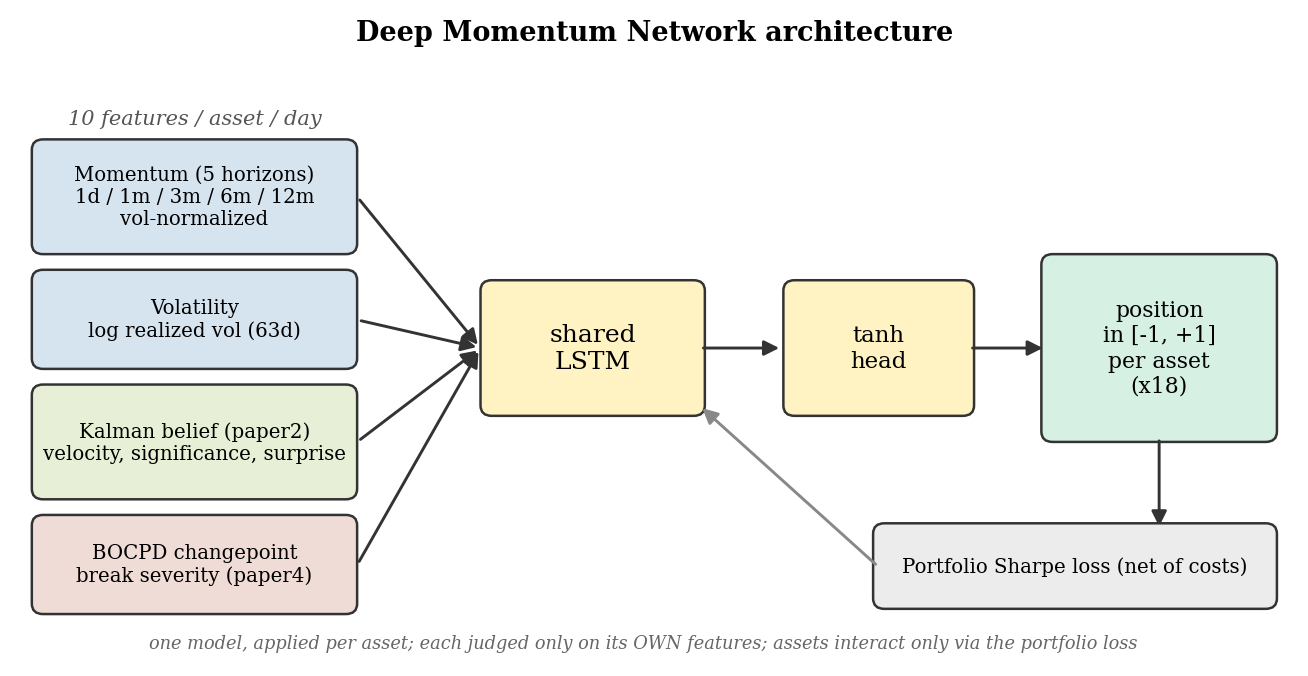
\includegraphics[width=.72\linewidth]{fig_architecture.png}
\caption{Οι καταστάσεις πεποίθησης (Kalman: ταχύτητα/σημαντικότητα/έκπληξη· BOCPD: σοβαρότητα) είναι
τέσσερις από τις δέκα εισόδους ανά προϊόν που τροφοδοτούν το LSTM.}\end{figure}

\section*{Τι να κρατήσετε}
\begin{itemize}[nosep,leftmargin=1.4em]
\item Δεν ταΐζουμε το μοντέλο με ωμές τιμές, αλλά με \textbf{καταστάσεις πεποίθησης} --- εκτιμήσεις για το τι συμβαίνει πίσω από την τιμή.
\item Το \textbf{Kalman} καθαρίζει τον θόρυβο και δίνει τάση \emph{και} βαθμό εμπιστοσύνης (σημαντικότητα τάσης), συν την «έκπληξη» της ημέρας.
\item Το \textbf{BOCPD} παρακολουθεί το μήκος διαδρομής· όταν η πιθανότητα καταρρέει στα μικρά μήκη, σημαίνει αλλαγή καθεστώτος (σοβαρότητα $\to 1$).
\item Μαζί δίνουν στο LSTM μια έτοιμη «εικόνα» τάσης και ρίσκου, αντί να την ψάχνει μόνο του μέσα στον θόρυβο.
\end{itemize}

\vfill
\noindent\rule{\linewidth}{0.4pt}\\[2pt]
{\small QUANTIQ / AGEL AI. Εκπαιδευτικό συνοδευτικό της εργασίας \emph{«From Dead Cross-Sectional
Momentum to Belief-State Deep Time-Series Momentum»} (Drakos 2026). Συνέχεια του φυλλαδίου για το LSTM.}

\end{document}
